The Matlab code used to generate the plots is shown below.
\begin{lstlisting}
% transfer functions for plants and controllers
P_lon = tf([1/(P.mc+2*P.mr)],[1,0,0]);
P_lat_in = tf([1/(P.Jc+2*P.mr*P.d^2)],[1,0,0]);
P_lat_out = tf([-P.Fe/(P.mc+2*P.mr)],[1,P.mu/(P.mc+2*P.mr),0]);
C_lon = tf([(P.kd_h+P.kp_h*P.sigma),...
            (P.kp_h+P.ki_h*P.sigma),P.ki_h],[P.sigma,1,0]);
C_lat_in = tf([(P.kd_th+P.sigma*P.kp_th), P.kp_th],...
              [P.sigma, 1]);
C_lat_out = tf([(P.kd_z+P.sigma*P.kp_z), P.kp_z],...
               [P.sigma, 1]);

% margin and bode plots for longitudinal controller 
figure(1), clf, margin(P_lon*C_lon), grid on, hold on
bode(P_lon*C_lon/(1+P_lon*C_lon)) 
legend('Open Loop-Inner', 'Closed Loop-Inner')

% margin and bode plots for lateral controller 
figure(2), clf, margin(P_lat_in*C_lat_in), grid on, hold on
bode(P_lat_in*C_lat_in/(1+P_lat_in*C_lat_in)) 
margin(P_lat_out*C_lat_out)
bode(P_lat_out*C_lat_out/(1+P_lat_out*C_lat_out))
legend('Open Loop-Inner', 'Closed Loop-Inner',...
       'Open Loop-Outer', 'Closed Loop-Outer')
\end{lstlisting}
The transfer functions for the longitudinal plant and controller are defined in Lines~2 and~5--6.  The {\tt margin} and {\tt bode} plots of the open and closed loop system respectively, for the longitudinal system are generated in Lines~12--15.
The results of this code are shown in Figure~\ref{fig:hw_vtol_altitude_margins}.
\begin{figure}[H]
   \centering
   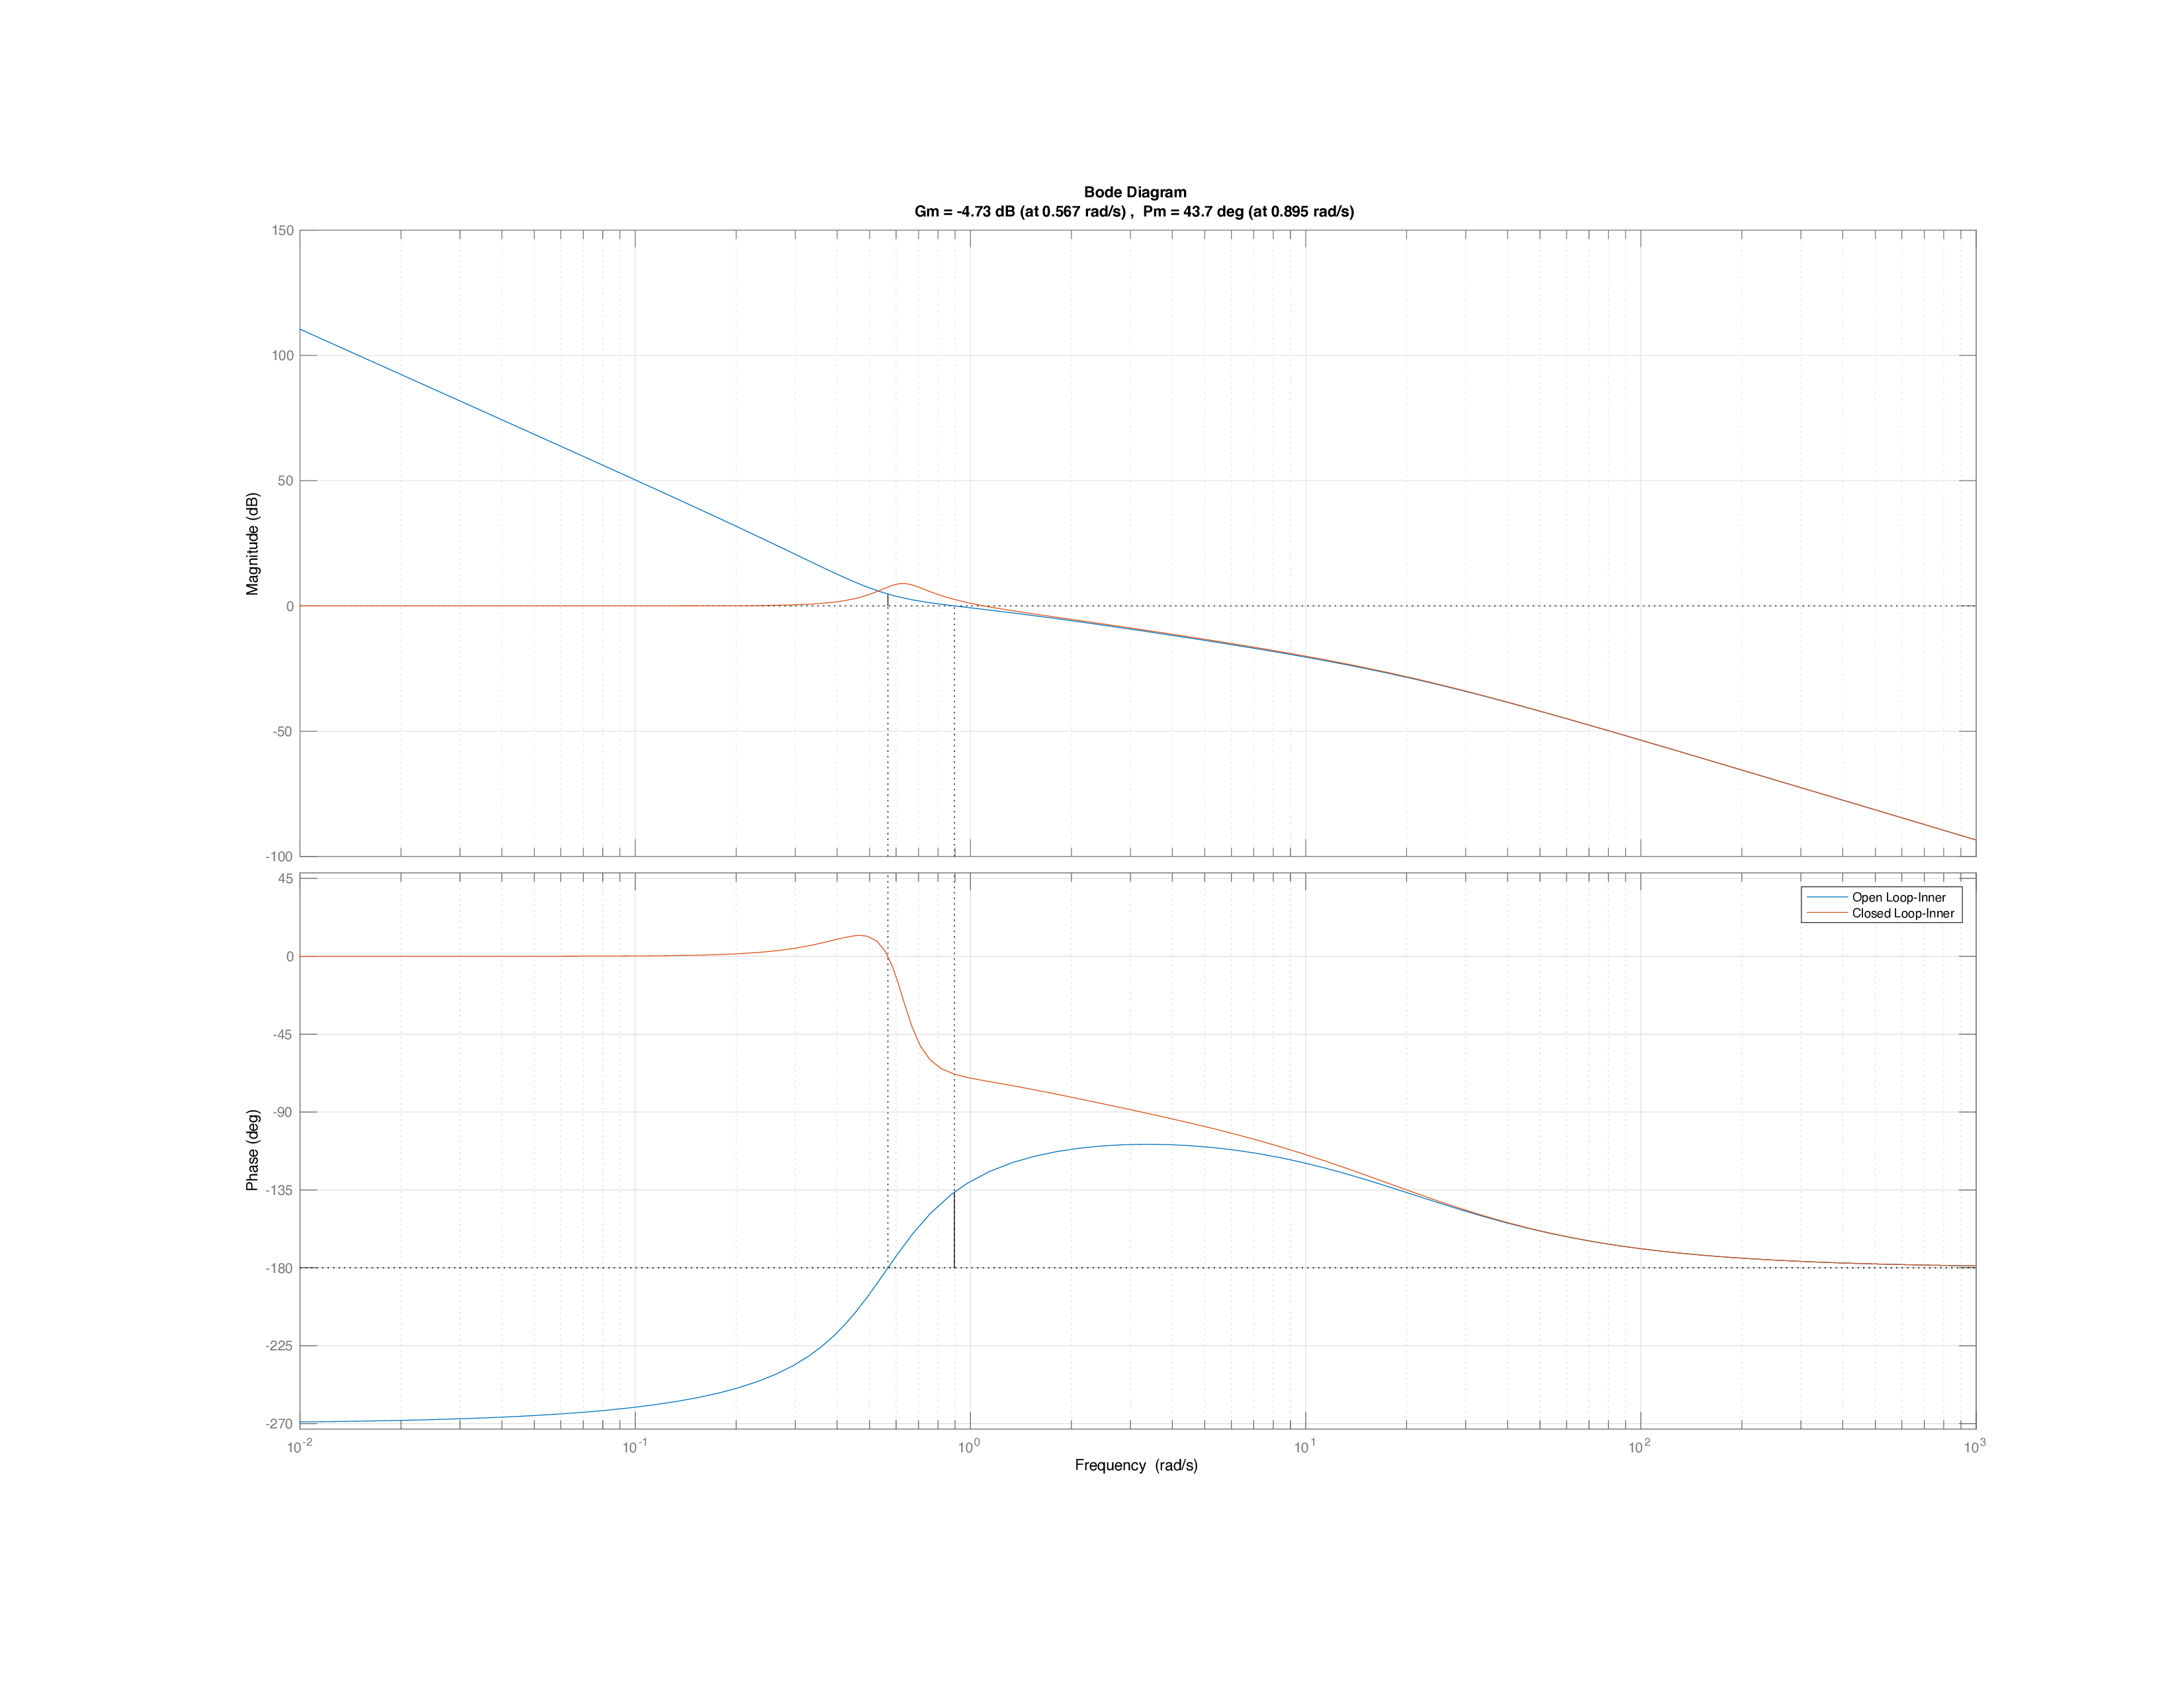
\includegraphics[width=0.95\textwidth]{6_design_studies/figures/hw_vtol_altitude_margins.pdf}
   \caption{The {\tt margin} plot of the open loop system and the {\tt bode} plot of the closed loop system, of the longitudinal control for the VTOL system under PID control.}
   \label{fig:hw_vtol_altitude_margins}
\end{figure} 

As seen from Figure~\ref{fig:hw_vtol_altitude_margins} the bandwidth of the closed loop system approximately $1.5$ whereas the cross over frequency is $0.9$~rad/sec.  We also see from  Figure~\ref{fig:hw_vtol_altitude_margins} that there is a resonance in the closed loop system at crossover.  This is due to the relatively small phase margin of $PM=43.7$~degrees. 


The transfer functions for the lateral inner and outer loop plants and controller are defined in Lines~3--4 and~7--10.  For this problem we plot both the inner and outer loop frequency response on the same Bode plot, as implemented in Lines~17--23. The results of this code are shown in Figure~\ref{fig:hw_vtol_lat_margins}.
\begin{figure}[H]
   \centering
   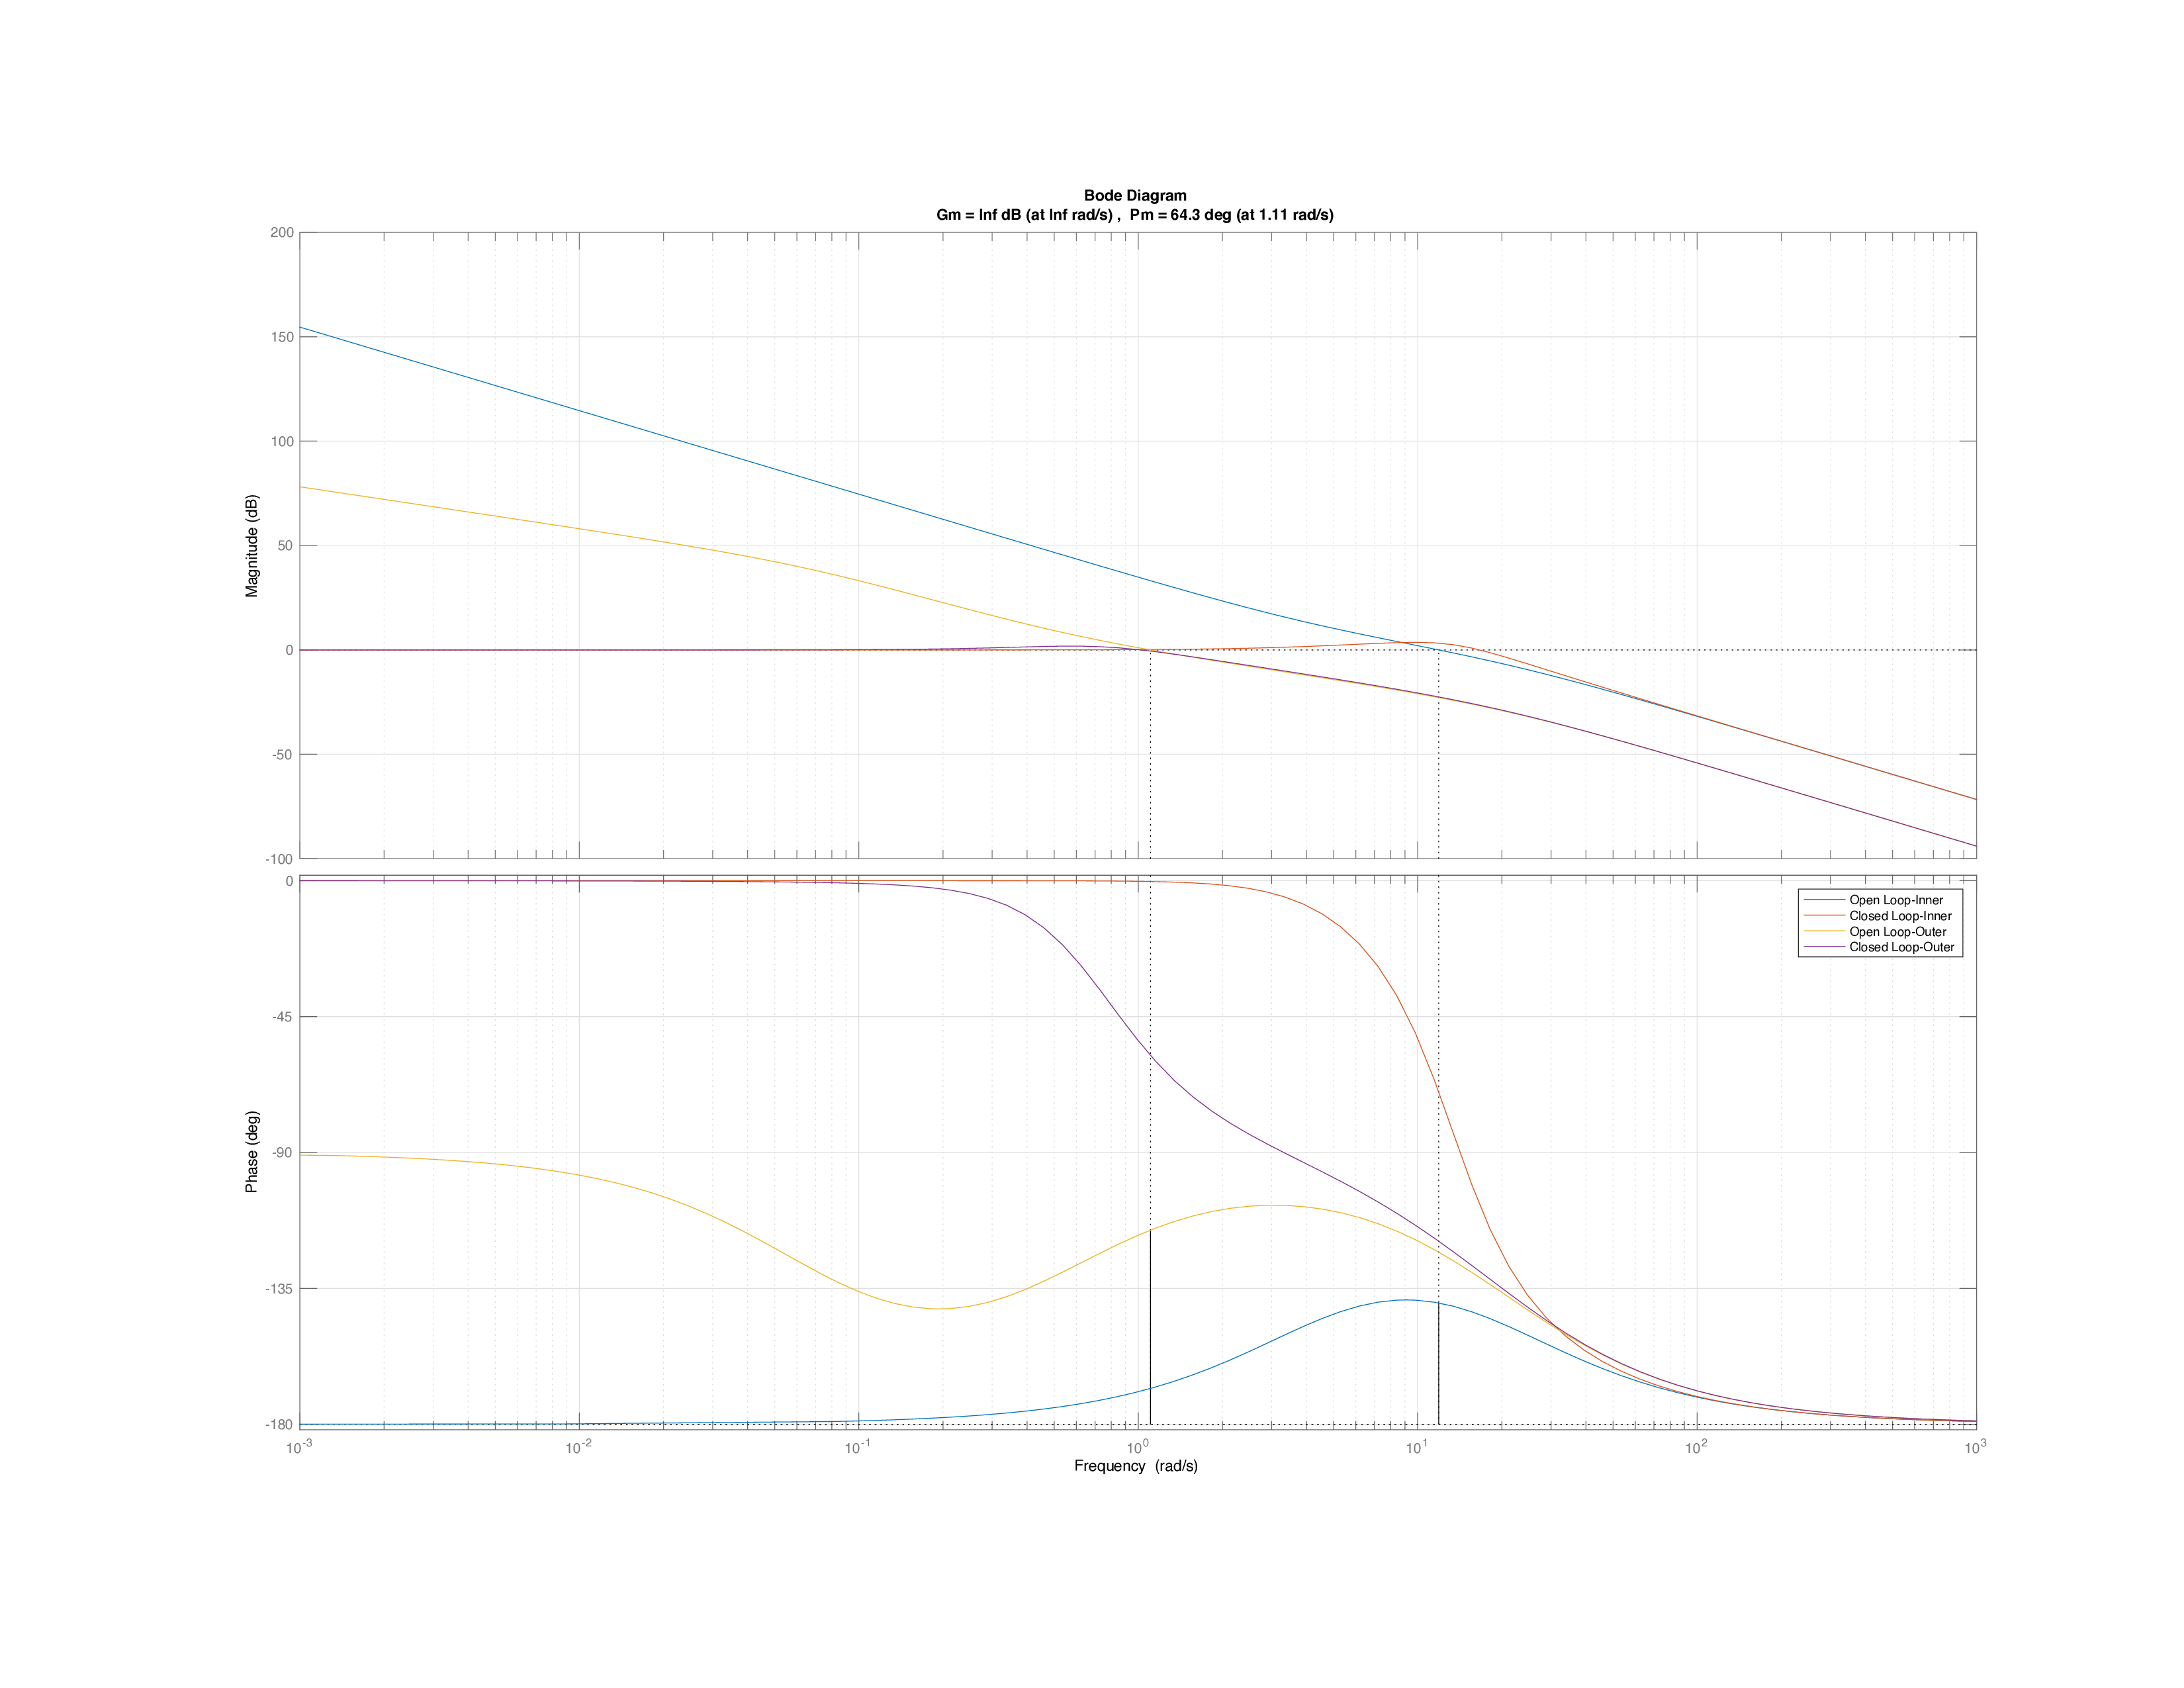
\includegraphics[width=0.95\textwidth]{6_design_studies/figures/hw_vtol_lat_margins.pdf}
   \caption{The {\tt margin} and {\tt bode} plots for the the open and closed loop systems of both the inner and outer loops of the VTOL lateral system.}
   \label{fig:hw_vtol_lat_margins}
\end{figure} 
As seen from Figure~\ref{fig:hw_vtol_lat_margins} the bandwidth of the inner loop is approximately $21$~rad/sec, which is larger than the cross over frequency of $12$~rad/sec.  The larger bandwidth is due to the small phase margin of $PM=41$~degrees.
%
Similarly, Figure~\ref{fig:hw_vtol_lat_margins} indicates that the bandwidth of the outer loop is approximately equal to $1.4$ where the cross over frequency is approximately $1.1$~rad/sec, due to the excellent phase margin of $PM=64.3$~degrees.

The bandwidth separation between the inner and outer loop is almost a decade and successive loop closure is justified by the fact that the bode plot of the inner loop is approximately one far beyond the cross over frequency of the outer loop.
